% july 2015
% Autor: Mandy Vogel
% linear modelling mainly from SPE 2011 M.Plummer

% \documentclass[xcolor={table},handout]{beamer}
 \documentclass[xcolor={table}]{beamer}
% \documentclass[xcolor={table},notes=show]{beamer}
% \usetheme[backgroundimagefile=mathe]{diepen}
\usetheme{Singapore}
\useoutertheme{miniframes}

%\setbeamerfont{block title}{size=\small,series=\bfseries}
%\setbeamerfont{block body}{size=\footnotesize}

% \usecolortheme{beetle}
%% \usepackage{linkimage}

%\usepackage{handoutWithNotes}
%\pgfpagesuselayout{3 on 1 with notes}[a4paper,border shrink=5mm]
%\pgfpagesuselayout{2 on 1}[a4paper,border shrink=5mm]

\begin{document}

\title{Linear Models}   
\author{Mandy Vogel} 
\date{\today}

% \AtBeginSection{
%   \begin{frame}<beamer>{Table of Contents}
%     \tableofcontents[currentsection]
%   \end{frame}}

\begin{frame}
\titlepage
\end{frame}

\begin{frame}{Table of Contents}
\frametitle{Table of Contents}\tableofcontents
\end{frame}

\section{Regression}

\begin{frame}\frametitle{The Null model}
\begin{columns}
\begin{column}{0.6\textwidth}
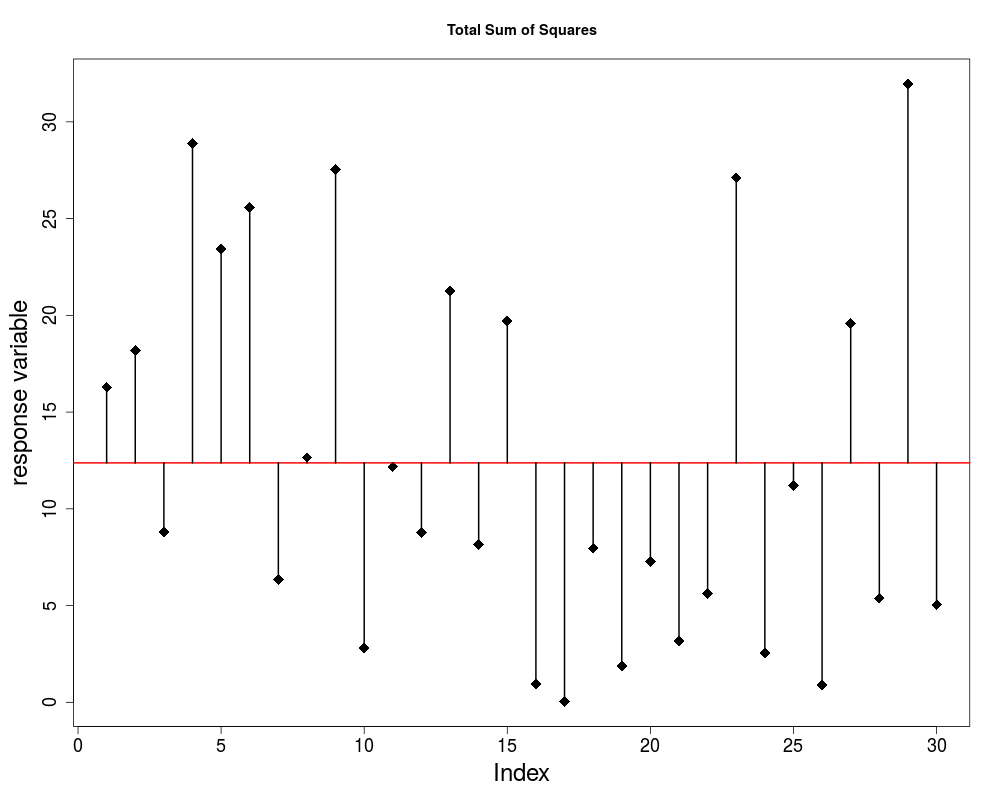
\includegraphics[width=6.5cm]{nullmodel.png}
\end{column}
\begin{column}{0.4\textwidth}
\begin{itemize}
\item Just one parameter, the overall mean $\bar{y}$
\item Fit: none; $SSE = SSY$
\item Degrees of freedom: $n-1$
\item Explanatory power of the model: none
\end{itemize}
\end{column}
\end{columns}
\end{frame}

\begin{frame}\frametitle{Adding Information}
\begin{columns}
\begin{column}{0.6\textwidth}
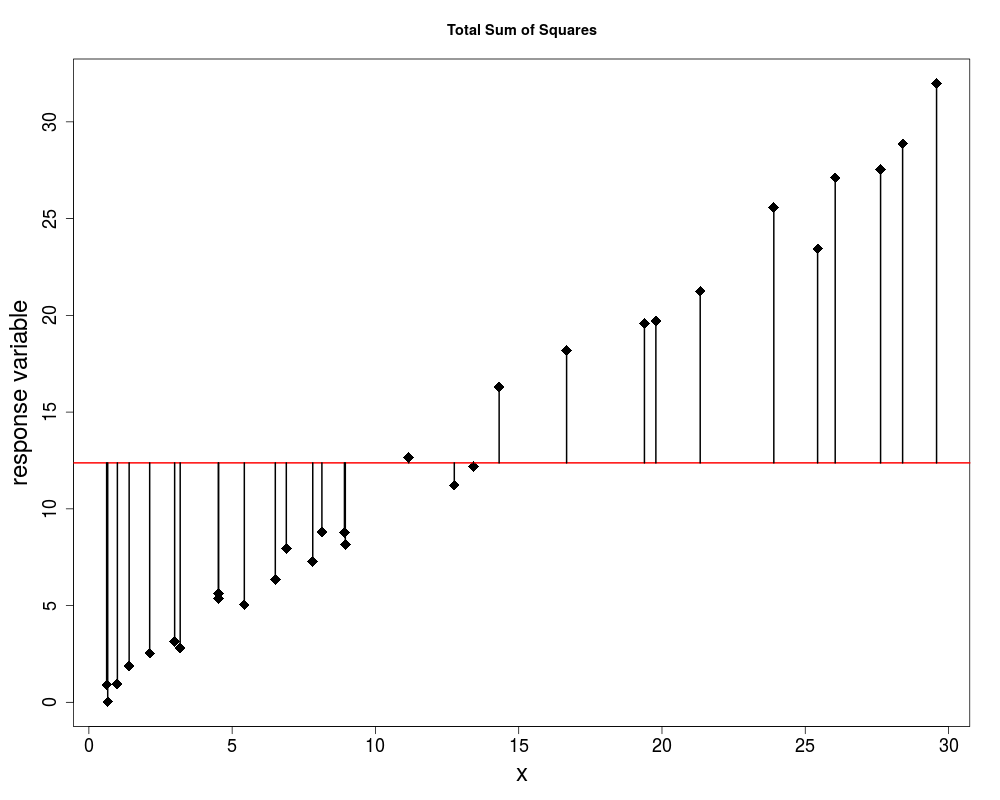
\includegraphics[width=6.5cm]{minimalmodel.png}
\end{column}
\begin{column}{0.4\textwidth}
\begin{itemize}
\item model with $0 \le p' \le p$ parameters
\item Fit: less than the maximal model, but not significantly so
\item Degrees of freedom: $n-p'-1$
\item Explanatory power of the model: $r^2 = \frac{SSR}{SSY}$    
\end{itemize}
\end{column}
\end{columns}
\end{frame}

\begin{frame}\frametitle{Adding Information}
\begin{columns}
\begin{column}{0.6\textwidth}
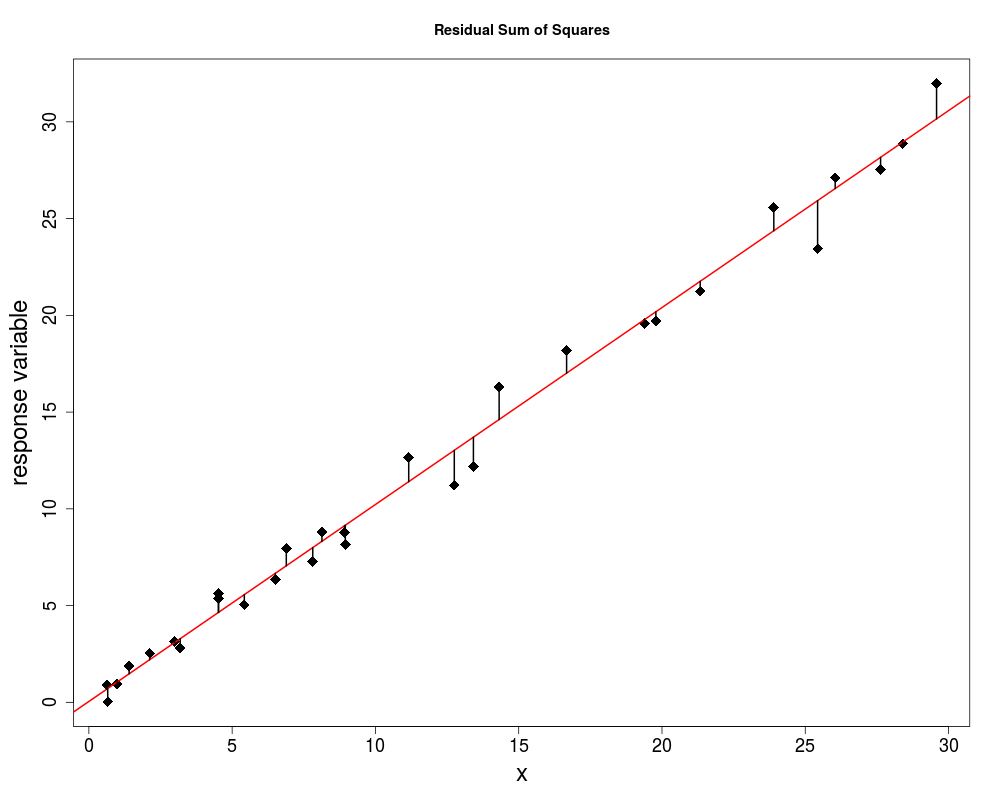
\includegraphics[width=6.5cm]{minimalmodel2.png}
\end{column}
\begin{column}{0.4\textwidth}
\begin{itemize}
\item model with $0 \le p' \le p$ parameters
\item Fit: less than the maximal model, but not significantly so
\item Degrees of freedom: $n-p'-1$
\item Explanatory power of the model: $r^2 = \frac{SSR}{SSY}$    
\end{itemize}
\end{column}
\end{columns}
\end{frame}


\section{Data}
\begin{frame}\frametitle{The births data}
A data frame with 500 observations on the following 8 variables. 
\begin{center}
\rowcolors{1}{gray!10}{gray!30}
\begin{tabular}{@{} >{\ttfamily}r l}
             id: & Identity number for mother and baby.               \\
       bweight: & Birth weight of baby.                              \\
         lowbw: & Indicator for birth weight less than 2500 g.       \\
       gestwks: & Gestation period.                                  \\
       preterm: & Indicator for gestation period less than 37 weeks. \\
        matage: & Maternal age.                                      \\
           hyp: & Indicator for maternal hypertension.               \\
           sex: & Sex of baby: 1:Male, 2:Female.                     \\
\end{tabular}
\end{center}
From: Michael Hills and Bianca De Stavola (2002). A Short Introduction
     to Stata 8 for Biostatistics, Timberlake Consultants Ltd URL:
     http://www.timberlake.co.uk
\end{frame}

\begin{frame}[fragile]\frametitle{Transform Data}
\small
\begin{semiverbatim}
> births <- transform(births,
+       lowbw = factor(lowbw, labels=c("normal","low")),
+       preterm = factor(preterm, labels=c("normal","preterm")),
+       hyp = factor(hyp, labels=c("normal","hyper")),
+       sex = factor(sex, labels=c("M","F")),
+       gest4 = cut(gestwks, breaks=c(20,35,37,39,45),
+       right=F))
\end{semiverbatim}
(The original and the corrected version are contained in the data folder.)
\end{frame}

\subsection{Variables}
\begin{frame}\frametitle{Variables in Models}
The response variable must be numeric. Main types are
\begin{itemize}
\item Metric (a measurement with units); the easiest case, we will begin with this
\item Binary (two values code 0/1) 
\item Count (aggregated data)
\item Failure (does the subject fail at end of follow up)
\end{itemize}
Explanatory variables can be
\begin{itemize}
\item Numeric
\item Factor
\end{itemize}
\end{frame}




\section{\texttt{lm()}}
\begin{frame}[fragile]\frametitle{Metric Response, Numeric explanatory variable}
Assuming that the relationship of \texttt{bweight} with \texttt{gestwks} is roughly linear we can find the linear effect on \texttt{bweight} of a unit increase in \texttt{gestwks} with

\begin{semiverbatim}
> m <- lm(bweight ~ gestwks, data=births)
\end{semiverbatim}

\begin{itemize}
\item \texttt{lm()} is the linear model function
\item \verb|bweight ~ gestwks| is the model formula
\item \texttt{m} is a model object (containing all information about our model), there are certain functions to extract these information, e.g.:
\end{itemize}

\begin{semiverbatim}
> coef(m)
(Intercept)     gestwks 
 -4489.1398    196.9726 
\end{semiverbatim}

One extra week of gestation produces an extra 197g of baby.
\end{frame}

\begin{frame}[fragile]\frametitle{Extractor functions}\footnotesize
\begin{semiverbatim}
> summary(m)

Call:
lm(formula = bweight ~ gestwks, data = births)

Residuals:
     Min       1Q   Median       3Q      Max 
-1698.40  -280.14    -3.64   287.61  1382.24 

Coefficients:
             Estimate Std. Error t value Pr(>|t|)    
(Intercept) -4489.140    340.899  -13.17   <2e-16 ***
gestwks       196.973      8.788   22.41   <2e-16 ***
---
Signif. codes:  0 ‘***’ 0.001 ‘**’ 0.01 ‘*’ 0.05 ‘.’ 0.1 ‘ ’ 1 

Residual standard error: 449.7 on 488 degrees of freedom
  (10 observations deleted due to missingness)
Multiple R-squared: 0.5073,	Adjusted R-squared: 0.5062 
F-statistic: 502.4 on 1 and 488 DF,  p-value: < 2.2e-16 
\end{semiverbatim}
\end{frame}


\begin{frame}[fragile]\frametitle{Extractor functions}\small
\begin{verbatim}
> coef(m)
(Intercept)     gestwks 
 -4489.1398    196.9726 
> confint(m)
                 2.5 %     97.5 %
(Intercept) -5158.9503 -3819.3293
gestwks       179.7054   214.2399
\end{verbatim}
\end{frame}


\begin{frame}\frametitle{Other Useful Functions}
The model object is a list of different elements each of which can be accessed separately (see \texttt{str(m)} for the full list).

Other useful functions:
\begin{itemize}
\item \texttt{print(m)} simple display
\item \texttt{plot(m)} produces various diagnostic plots based on residuals
\item \texttt{fitted(m)} returns a vector of fitted values
\item \texttt{resid(m)} returns a vector of residuals
\item \texttt{predict(m, newdata)} predicts the response for new values of the explanatory variables
\item \texttt{deviance(m)} residual sum of squares
\item \texttt{df.residual(m)} for the residual degrees of freedom
\item \texttt{vcov(m)} variance-covariance matrix
\end{itemize}
\end{frame}



\begin{frame}[fragile]\frametitle{Explanatory Variable is a Factor}
The effect of \texttt{hyp} (2-level factor) on \texttt{bweight} is obtained with
\begin{verbatim}
> m <- lm(bweight ~ hyp, data=births)
> coef(m)
(Intercept)    hyphyper 
  3198.9042   -430.6959 
\end{verbatim}
Omitting the intercept gives the mean \texttt{bweight} at the two levels of \texttt{hyp}
\begin{verbatim}
> m <- lm(bweight ~ -1 + hyp, data=births)
> coef(m)
hypnormal  hyphyper 
 3198.904  2768.208
\end{verbatim}
\end{frame}


\begin{frame}[fragile]\frametitle{A Multivariable Model}
The joint effect of \texttt{hyp} and \texttt{gestwks} on \texttt{bweight} is obtained with
\begin{verbatim}
> m <- lm(bweight ~ hyp + gestwks, data=births)

             Estimate 
(Intercept) -4285.002 
hyphyper     -143.675 (level 2 vs. level 1)
gestwks       192.238 (increase per week)
\end{verbatim}

The effect of \texttt{hyp} is attenuated (from $-430.7$ to $-143.7$ ). This suggests that much of the effect of hypertension on birth weight is mediated through a shorter gestation period.
\end{frame}

\begin{frame}[shrink=5]\frametitle{A Model With Both \texttt{gestwks} and  \texttt{hyp}}
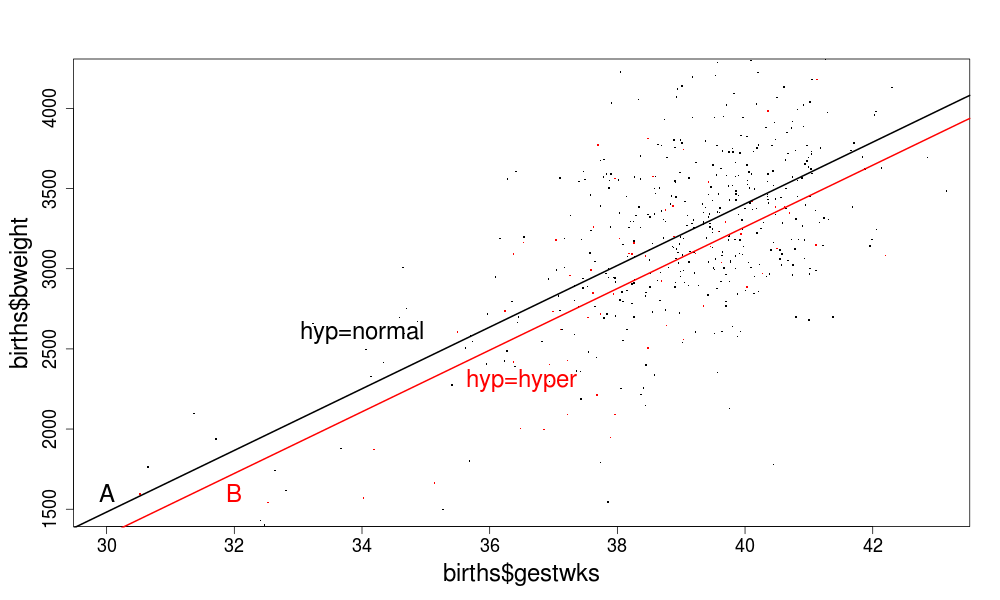
\includegraphics[height=7cm]{model1.png}

The effect of \texttt{gestwks} is the slope of the lines A and B (assumed to be the same). The effect of \texttt{hyp} ist the vertical distance between them.
\end{frame}


\begin{frame}[fragile]\frametitle{Interaction Models in \texttt{lm}}
To specify an interaction term in \texttt{lm}, change the model formula from
\begin{exampleblock}{Input}\small
\begin{semiverbatim}
> m <- lm(bweight ~ hyp + gestwks, data=births)
\end{semiverbatim}
to
\begin{semiverbatim}
> m <- lm(bweight ~ hyp + gestwks + hyp:gestwks, data=births)
\end{semiverbatim}
or shorter
\begin{semiverbatim}
> m <- lm(bweight ~ hyp * gestwks, data=births)
\end{semiverbatim}
\end{exampleblock}
\end{frame}


\begin{frame}[shrink=5]\frametitle{Interaction Between \texttt{gestwks} and  \texttt{hyp}}
\begin{center}
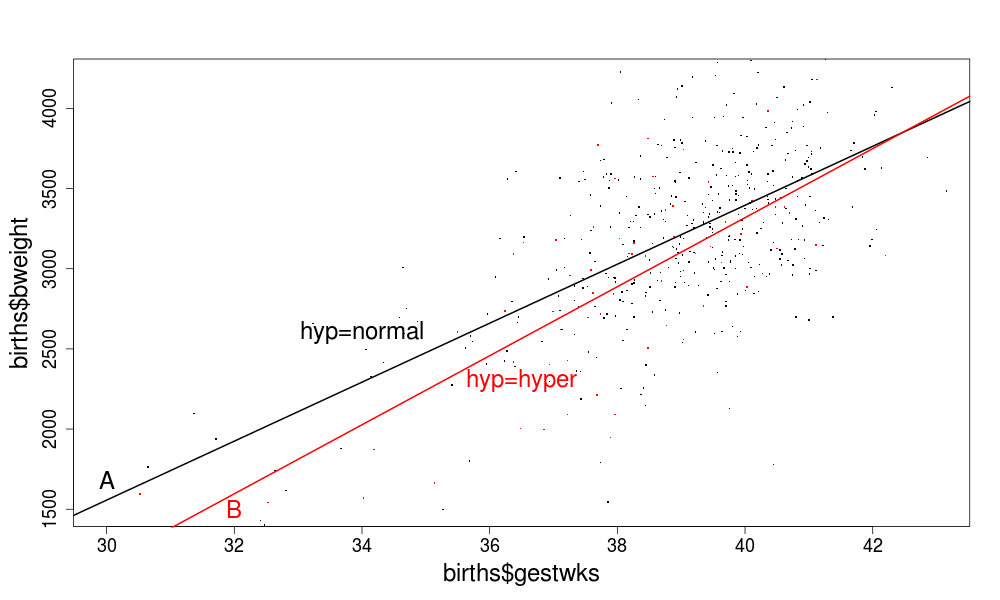
\includegraphics[height=8cm]{model2.png}
\end{center}
\end{frame}


\begin{frame}[fragile]\frametitle{Interactions Models in \texttt{lm}}
\begin{exampleblock}{Output}
\begin{semiverbatim}
                 Estimate
(Intercept)      -3960.82
hyphyper         -1332.66 (level 2 vs level 1 - intercept)
gestwks            183.91
hyphyper:gestwks    31.39 (level 2 vs level 1 - slope)
\end{semiverbatim}
\end{exampleblock}
Now the effect of \texttt{hyp} more difficult to explain, because it is not constant. The effect of  $-1332$ is valid on a hypothetical gestational age of $0$. Which doesn't make sense. You could scale the \texttt{gestwks} variable. 
\begin{semiverbatim}
> births$gwsc <- births$gestwks-40
> m <- lm(bweight ~ hyp * gwsc, data=births)
\end{semiverbatim}
\end{frame}

\begin{frame}[fragile]\frametitle{Interactions Models in \texttt{lm}}
\begin{exampleblock}{Input/Output}
\begin{semiverbatim}
                Estimate
(Intercept)   3395.60329 
hyphyper       -77.25215 (level 2 vs level 1 - intercept)
gwsc           183.91048
hyphyper:gwsc   31.38510 (level 2 vs level 1 - slope)
\end{semiverbatim}
\end{exampleblock}
\end{frame}

\begin{frame}[fragile]\frametitle{How much is explained? - aov}
In the Null-Model we have seen that $SSE=SSY$ (the error sum of squares is equal to the total sum of squares in y) and therefore the Null-Model explaines nothing of the overall variance. So the fraction how much of the overall variance is explained by our model regarding to the overall variance is a first measure for the fit of the model...
\begin{itemize}
\item the simple model with one explanatory variable\small
\begin{semiverbatim}
> m <- lm(bweight ~ gestwks, data=births)
> anova(m)
Analysis of Variance Table

Response: bweight
           Df    Sum Sq   Mean Sq F value    Pr(>F)    
gestwks     1 101603845 101603845  502.36 < 2.2e-16 ***
Residuals 488  98698698    202251                      
---
Signif. codes:  0 ‘***’ 0.001 ‘**’ 0.01 ‘*’ 0.05 ‘.’ 0.1 ‘ ’ 1 
\end{semiverbatim}
\end{itemize}
\end{frame}


\begin{frame}[fragile]\frametitle{How much is explained? - aov}
\begin{itemize}
\item in the second column of the summary we see the regression sum of squares ( $SSR$ ) in the first line and in the second line the error sum of squares ($SSE$ ). So the total sum of squares ( $SSY$ - a measure for the overall variation) is the sum of both:
\begin{verbatim}
> sum(anova(m)$Sum)
[1] 200302543
\end{verbatim}
\item and the fraction is
\begin{verbatim}
> anova(m)$Sum[1]/sum(anova(m)$Sum)
[1] 0.5072519
\end{verbatim}
\end{itemize}
\end{frame}

\begin{frame}[fragile]\frametitle{How much is explained? - aov}
\begin{itemize}
\item this is r-squared 
\begin{verbatim}
> summary(m)$r.squared
[1] 0.5072519
\end{verbatim}
\item which you can extract from the summary of the model\footnotesize
\begin{verbatim}
> summary(m)
Call:
lm(formula = bweight ~ gestwks, data = births)
Residuals:
     Min       1Q   Median       3Q      Max 
-1698.40  -280.14    -3.64   287.61  1382.24 
Coefficients:
             Estimate Std. Error t value Pr(>|t|)    
(Intercept) -4489.140    340.899  -13.17   <2e-16 ***
gestwks       196.973      8.788   22.41   <2e-16 ***

Residual standard error: 449.7 on 488 degrees of freedom
  (10 observations deleted due to missingness)
Multiple R-squared: 0.5073,	Adjusted R-squared: 0.5062 
F-statistic: 502.4 on 1 and 488 DF,  p-value: < 2.2e-16 
\end{verbatim}
\end{itemize}
\end{frame}

\begin{frame}[fragile,allowframebreaks]\frametitle{Exercises}
  \begin{enumerate}
  \item load the nhanes data
  \item how many observations, how many variables?
  \item how old are the participants (summary statistics, mean, sd)
  \item plot waist circumference vs age
  \item model the respective data in a linear model, extract and interpret the coefficients. Extract also the confidence intervals.
  \item add sex as a covariate. interpret. 
  \end{enumerate}
  
\end{frame}


\section{\texttt{glm}}
\begin{frame}[fragile]\frametitle{Generalized Linear Models}
\begin{exampleblock}{Input}
\begin{semiverbatim}
> m <- lm(bweight ~ hyp, data=births)
> m <- glm(bweight ~ hyp, family=gaussian, data=births)
\end{semiverbatim}
\end{exampleblock}

give the same answer. The model formula is the same for both, but for \texttt{glm} it is necessary to specify the family of likelihoods which will be used to fit the model. 

The \texttt{glm} function allows us to fit other models including logistic regression and Poisson regression.
\end{frame}

\begin{frame}[fragile]\frametitle{Predicting Low Birth Weight}
We are more interested in predicting birth weight under 2500g (\texttt{lowbw}). This requires a model where the outcome is not metric, but binary. For a binary response we use a \texttt{glm} with a \emph{binomial} family.
\begin{exampleblock}{Input/Output}\note{lacks interpretation (10.3 = 40/388)}
\begin{semiverbatim}\small
> m <- glm(lowbw ~ hyp, family=binomial, data=births)
> ci.lin(m, Exp=T)[,5:7]
            exp(Est.)       2.5%     97.5%
(Intercept) 0.1030928 0.07445162 0.1427521
hyphyper    3.7307692 2.02747522 6.8650107
\end{semiverbatim}
\end{exampleblock}
This returns estimates of the log odds (Intercept) or log odds ratios (for the parameters). To present the results in terms of odds ratios we use the \verb|Exp=TRUE| option to \texttt{ci.lin}.
\end{frame}

\begin{frame}[fragile]\frametitle{Controlling}
Controlling the effect of \texttt{hyp} on \texttt{lowbw} for \texttt{sex}
\begin{exampleblock}{Input/Output}\note{lacks interpretation}
\begin{semiverbatim}\small
> m <- glm(lowbw ~ hyp+sex, family=binomial, data=births)
> ci.lin(m,Exp=T)
              exp(Est.) 
(Intercept)   0.0813691 
hyphyper      3.9060041 (\texttt{hyp} controlled for \texttt{sex})
sexF          1.5641095 (\texttt{sex} controlled for \texttt{hyp})
\end{semiverbatim}
\end{exampleblock}
When you control for a variable you are assuming that any interaction can be ignored.
\end{frame}


\begin{frame}[fragile]\frametitle{Interaction (effect modification)}
\begin{exampleblock}{Input/Output}\note{lacks interpretation}
\begin{semiverbatim}
> m <- glm(lowbw ~ hyp + sex + hyp:sex, 
+           family=binomial, data=births)
> ci.lin(m,Exp=T)[,5:7]
               exp(Est.)
(Intercept)   0.07281553
hyphyper      5.31612903
sexF          1.88644689
hyphyper:sexF 0.52168285 
\end{semiverbatim}
\end{exampleblock}
Alternatively, use
\begin{exampleblock}{Input/Output}
\begin{semiverbatim}
m <- glm(lowbw ~ hyp*sex, family=binomial, data=births)
\end{semiverbatim}
\end{exampleblock}

\end{frame}


\begin{frame}[fragile]\frametitle{Testing for Interaction}
\begin{exampleblock}{Input/Output}\note{lacks interpretation}
\begin{semiverbatim}
> m1 <- glm(lowbw ~ hyp+sex, family=binomial, data=births)
> m2 <- glm(lowbw ~ hyp*sex, family=binomial, data=births)
> anova(m1,m2,test="Chisq")

  Resid. Df Resid. Dev Df Deviance Pr(>Chi)
1       497     348.34                     
2       496     347.29  1   1.0561   0.3041
\end{semiverbatim}
\end{exampleblock}
The \texttt{anova} function conducts an \emph{analysis of variance} -- an old-fashioned name for a test of significance between two nested models.
\end{frame}


\begin{frame}[fragile]\frametitle{Stratified Effects}
When there is a strong interaction it may be best to report stratified effects. Omitting the main effect of \texttt{hyp} in an interaction model gives us the effect of \texttt{hyp} within strata of \texttt{sex}.
\begin{exampleblock}{Input/Output}\note{lacks interpretation}
\begin{semiverbatim}
m <- glm(lowbw ~ sex + sex:hyp, family=binomial, 
+                               data=births)
> ci.lin(m,Exp=T)[,5:7]
               exp(Est.)
(Intercept)   0.07281553 % 15/206 nur normale Jungen
sexF          1.88644689
sexM:hyphyper 5.31612903
sexF:hyphyper 2.77333333
\end{semiverbatim}
\end{exampleblock}
Note that $2.77/5.32=0.52$ is the interaction term.
\end{frame}



\begin{frame}\frametitle{Looking Inside the Black Box}
The paradigm is the model
$$\mu = \alpha + \beta X + \gamma Z + \cdots$$

where $X$,$Z$,$\cdots$ are numeric explanatory variables. In a glm $\mu$ is replaced by some function of $mu$ such as $\log(\mu)$ (link function). 

When $X$ is a factor, on (say) 3 levels, it is replaced by $X_1,X_2,X_3$, die indicator variables for the levels of $X$.

Predicted values for $\alpha+\beta_1X_1+\beta_2X_2+\beta_3X_3 $ are

\vspace*{0.5cm}

\begin{center}
\begin{tabular}{l c c c c}
level&$X_1$&$X_2$&$X_3$&$\alpha+\beta_1X_1+\beta_2X_2+\beta_3X_3 $\\
\hline
1&1&0&0&$\alpha+\beta_1$\\
2&0&1&0&$\alpha+\beta_2$\\
3&0&0&1&$\alpha+\beta_3$\\
\end{tabular}
\end{center}

\end{frame}



\begin{frame}[shrink=2]\frametitle{Too Many Parameters}
Drop $\alpha$

\begin{center}
\begin{tabular}{l c c c c}
level&$X_1$&$X_2$&$X_3$&$\beta_1X_1+\beta_2X_2+\beta_3X_3 $\\
\hline
1&1&0&0&$\beta_1$\\
2&0&1&0&$\beta_2$\\
3&0&0&1&$\beta_3$\\
\end{tabular}
\end{center}

$\beta_1$ is the mean response at level 1, $\beta_2$ at level 2, $\beta_3$ at level 3.

Drop $X_1$

\begin{center}
\begin{tabular}{l c c c}
level&$X_2$&$X_3$&$\alpha+\beta_2X_2+\beta_3X_3 $\\
\hline
1&0&0&$\alpha$\\
2&1&0&$\alpha+\beta_2$\\
3&0&1&$\alpha+\beta_3$\\
\end{tabular}
\end{center}

$\alpha$ is the mean response at level 1

$\beta_2$ und $\beta_3$ are the effects of levels 2 and 3 vs level 1. These are called \emph{treatment contrasts}.

\end{frame}


\begin{frame}[shrink=2]\frametitle{Two Factors}
$X$ on 3 levels, $Z$ on 2 levels

$$\mu=\alpha+\beta_1X_1+\beta_2X_2+\beta_3X_3+\gamma_1Z_1+\gamma_2Z_2$$ 

$X_1,X_2,X_3$ are the indicators for $X$ and $Z_1,Z_2$ are the indicators for $Z$. Omitting $X_1$ and $Z_1$ the model becomes

$$\mu=\alpha+\beta_2X_2+\beta_3X_3+\gamma_2Z_2$$ 

with predicted means

\begin{center}
\begin{tabular}{c c c c}
&&\multicolumn{2}{c}{$Z$}\\
&&1&2\\
\hline
   &1&$\alpha$&$\alpha+\gamma_2$\\
$X$&2&$\alpha+\beta_2$&$\alpha+\beta_2+\gamma_2$\\
   &3&$\alpha+\beta_3$&$\alpha+\beta_3+\gamma_2$\\
\end{tabular}
\end{center}
\end{frame}


\begin{frame}[shrink=2]\frametitle{Interaction}
Effect of $Z$ the same at each level of $X$:

\begin{center}
\begin{tabular}{c c c c}
&&\multicolumn{2}{c}{$Z$}\\
&&1&2\\
\hline
   &1&$\alpha$&$\alpha+\gamma_2$\\
$X$&2&$\alpha+\beta_2$&$\alpha+\beta_2+\gamma_2$\\
   &3&$\alpha+\beta_3$&$\alpha+\beta_3+\gamma_2$\\
\end{tabular}
\end{center}

Effect of $Z$ differs at different levels of $X$:

\begin{center}
\begin{tabular}{c c c c}
&&\multicolumn{2}{c}{$Z$}\\
&&1&2\\
\hline
   &1&$\alpha$&$\alpha+\gamma_2$\\
$X$&2&$\alpha+\beta_2$&$\alpha+\beta_2+\gamma_2+\delta_{22}$\\
   &3&$\alpha+\beta_3$&$\alpha+\beta_3+\gamma_2+\delta_{32}$\\
\end{tabular}
\end{center}

The $\delta$ parameters measure how much the effect of $Z$ changes.
\end{frame}



\begin{frame}[fragile]\frametitle{Nested or Stratified Effects}

A slightly different way of parameterizing the model gives stratified effects:

\begin{center}
\begin{tabular}{c c c c}
&&\multicolumn{2}{c}{$Z$}\\
&&1&2\\
\hline
   &1&$\beta_1$&$\beta_1\delta_{12}$\\
$X$&2&$\beta_2$&$\beta_2+\delta_{22}$\\
   &3&$\beta_3$&$\beta_3+\delta_{32}$\\
\end{tabular}
\end{center}

Same number of parameters as for interaction, but the $\delta$`s now measure the effects of $Z$ at each level of $X$. In \texttt{R} this would be produced by the model formula \verb|Y ~ -1 + X + X:Z |

\end{frame}


%% XXX Alternatives to treatment contrasts lacks 2 slides

\end{document}

